\begin{slikaDesno}{fig/comb_RLC.pdf}
\PID 
У колу приказаном на слици познато је 
$L = 1\unit{\upmu H}$, $C = 1\unit{\upmu F}$,  
и 
$R = 10\unit{k\Omega}$. 
Једини улаз посматраног система је струја 
$i_{\rm G} = i_{\rm G}(t)$, а једини излаз
је напон $v_{\rm I} = v_{\rm I}(t)$. 
сматрати да је 
$\sqrt{LC} \gg \dfrac{L}{R}$.
\begin{enumerate} [label=(\alph*)]  
    \item Одредити импулсни одзив датог система,
    $h(t)$, и скицирати његов график.  
\end{enumerate}
\end{slikaDesno}

\begin{enumerate}[label=(\alph*)]  
    
    \stepcounter{enumi}
    
    \item Одредити сопствени одзив датог система, ако  
    су $v_{\rm I}(0^-) = 2\unit{V}$ и $\dfrac{\de v_{\rm I}}{\de t}
    (0^-)
    = 1 \unit{\dfrac{V}{ms}}$.

    \item Дати систем се користи за реализацију
    осцилатора (уређаја који гененерише осцилације), заснованог на природном понашању 
    $LC$ кола, док отпорност $R$
    моделује неизбежне губитке. Улаз система 
    (струја струјног  извора) се може користити
    да те губитке надокнади, додавањем 
    одређене количине наелектрисања у сваком 
    периоду током веома кратког времена. Тај 
    процес  се може представити као 
    $i_{\rm G}(t) = Q\, \text{Ш}_{T_0}(t)$, где $T_0$ 
    одговара периоду простопериодичнног члана 
    хомогеног дела одзива. 
    Приближно одредити зависност амплитуде (максималне тренутне 
    вредности) устаљеног одзива система од количине наелектрисања $Q$.
\end{enumerate}
    
\RESENJE

(а) Диференцијална једначина система 
налази се писањем Кирхофовог закона за 
струје у задатом колу као 
$
i_{\rm G} = \underbrace{C\dfrac{\de v_C}{\de t}}_{i_C} 
            + i_L
            + \underbrace{\dfrac{v_I}{R}}_{i_R}.
$
Додатним диференцирањем обе стране једнакости по времену па затим сређивањем даље се има 
погодан облик 
\begin{eqnarray}
    \dfrac{\de i_{\rm G}}{\de t} = 
    C\dfrac{\de^2 v_I}{\de t^2} 
    + \dfrac{\de i_L}{\de t}
    + \dfrac{1}{R} \dfrac{\de v_I}{\de t} 
    \qquad 
    \Rightarrow
    \qquad
    L \dfrac{\de i_{\rm G}}{\de t} = 
    LC\dfrac{\de^2 v_I  }{\de t^2} 
    + \dfrac{L}{R} \dfrac{\de v_{\rm I}}{\de t} 
    + v_{\rm I}
\end{eqnarray}
Добијена диференцијална једначина се 
може представити и у операторском 
облику као 
\begin{equation}
    P({\rm D}) v_{\rm I}
    =
    Q({\rm D}) i_{\rm G} 
     , 
    \qquad
    Q({\rm D}) = L, \qquad
    P({\rm D}) = LC\,{\rm D}^2 + 
    \dfrac{L}{R}\, {\rm D} + 1.
\end{equation}
Ради поједностављења записа, уведимо смене 
у виду временских параметара 
$T^2 = LC = 1\unit{\upmu s}$ и $\uptau = L/R = 100\unit{ps}$, 
па је онда каракеристични полином диференцијалне једначине система
$P(\uplambda) = T^2\,{\rm D}^2
+ \uptau\,{\rm D} + 1$, чији су одговарајући корени 
\begin{equation}
    \uplambda_{1,2} = \dfrac{-\uptau^2 \pm \sqrt{\uptau^4 - 4T^2} }{2T^2}.
\end{equation}
Пошто је $T \gg \uptau$ онда се може писати 
$
    \uplambda_{1,2} = \dfrac{-\uptau^2}{2T^2} \pm \dfrac{\sqrt{ \cancelto{\ll T^2}{\uptau^2} - 4T^2 }}{2T^2} 
    \approx  \dfrac{-\uptau^2}{2T^2} \pm \dfrac{\overbrace{\sqrt{ - 4T^2 }}^{\jj 2T } }{2T^2}
    = - \dfrac{\uptau^2}{2T^2} \pm \jj\dfrac{1}{T}. 
$ Заменом израза за $\uptau$ и $T$ добијају се корени у облику 
\begin{equation}
    \uplambda_{1,2} \approx \upsigma \pm \jj \upomega, \quad
    \upsigma = -\dfrac{\uptau}{2T^2} 
    = -\dfrac{L/R}{2LC} = - \dfrac{1}{2RC}, 
    \qquad
    \upomega = \dfrac{1}{T} = \dfrac{1}{\sqrt{LC}}.
\end{equation}
Заменом бројних вредности налази се $\upsigma = -50\unit{s^{-1}}$ и $\upomega = 1\unit{\dfrac{Mrad}{s}}$.

Импулсни одзив датог система одређјује на начин описан у додатку 
\ref{a:impulsni_odziv}, решавањем помоћне 
једначине $\updelta(t) = P({\rm D}) p(t)$, па је онда 
$h(t) = Q({\rm D})p(t)$. Облик решења помоћне једначине је 
изграђен од карактеристичних фунцкија које потичу од 
коренова карактеристичног полинома па је облика
\begin{equation}
p(t) = {\rm e}^{\upsigma t} \left( A\sin(\upomega t) + 
B \cos(\upomega t) \right).
\end{equation}
Постиницијални услови услед Дираковог импулса су 
$p(0^+) = 0$, $p'(0^+) = \dfrac{1}{T^2}$, па је онда 
\begin{equation}
	p(0) = {\rm e^{\upsigma\cdot 0}}
	\left(A\sin(\upomega \cdot 0) + B\cos(\upomega\cdot 0)\right)
	= B \Rightarrow B = 0
\end{equation}
Диференцирањем остатка решења се налази 
\begin{equation}
	\dfrac{\de p}{\de t}
	= 
	A\left(
	\upsigma {\rm e}^{\upsigma t} \sin(\upomega t)
	+
	\upomega {\rm e}^{\upsigma t} \cos(\upomega t)
	\right)
	=
	A {\rm e}^{\upsigma t}
	\left(
	\upsigma \sin(\upomega t)
	+
	\upomega \cos(\upomega t)
	\right) 
\end{equation}
Одговарајућом заменом се онда налази 
\begin{equation}
	\dfrac{\de p}{\de t}(t = 0)
	= A\upomega = \dfrac{1}{T^2} 
	\Rightarrow A = \dfrac{1}{\upomega T^2} = 
	\dfrac{1}{T}.
\end{equation}
Коначно, импулсни одзив се налази као 
\begin{equation}
	h(t) = L \dfrac{\de p}{\de t}
	\Rightarrow	
	h(t) = 
	\dfrac{L}{T}
	{\rm e}^{\upsigma t}
	\bigg(
	\upsigma \sin(\upomega t)
	+
	\upomega \cos(\upomega t)
	\bigg) 	
	=
	\sqrt{\dfrac{L}{C}}\,
	\bigg(
	\upsigma \sin(\upomega t)
	+
	\upomega \cos(\upomega t)
	\bigg) 	
	{\rm e}^{\upsigma t}, 
\end{equation}
Заменом бројних вредности, апроксимацијом да је $\upomega\gg\upsigma$, 
и узимањем у обзир област важења импулсног одзива $t>0$, коначно је\footnote{
 Побуда за коју одзив има димензију напона је облика $Q\updelta(t)$, тако да побуда $\updelta(t)$ даје 
 одзив који се природно може изразити у јединици која је однос напона и наелектрисања, а има физички смисао
 напона по јединици наелектрисања у импулсу побуде. 
}
\begin{equation}
    h(t) = \ee^{-50\unit{s^{-1}}t } \cos(\upomega t) \uu(t) \unit{\dfrac{V}{\upmu C}}    
\end{equation}

(в) Озив на побуду може се изразити конволуцијом са импулсним одзивом, па се применом својстава
конволуције добија
\begin{eqnarray}
    v_{\rm I}(t) &=& i_{\rm G}(t) \ast h(t) = Q\, \text{Ш}_{T_0}(t) \ast \dfrac{1}{C} \ee^{\upsigma t} \cos(\upomega t)
                 \\ &=& \dfrac{Q}{C} \left(
                    \sum_{k = -\infty}^{\infty} \updelta(t - kT_0) \ast \ee^{\upsigma t} \cos(\upomega t) \uu(t)
                 \right) 
                 \\ &=& 
                 \dfrac{Q}{C} 
                 \sum_{k = -\infty}^{\infty} \left( \ee^{\upsigma(t - kT_0)} \uu(t - kT_0) 
                  \cos\big(\upomega (t - kT_0) \big) \right) 
                \\ &=& 
                \underbrace{    \dfrac{Q}{C} 
                 \sum_{k = -\infty}^{\infty} 
                 \left( \ee^{\upsigma(t - kT_0)} \uu(t - kT_0) 
                \right)}_{V_{\rm m}(t)}  \cos\big(\upomega t \big),
\end{eqnarray}
при чему је у последњем кораку употребљена периодичност косинусне функције 
$\cos\big(\upomega (t - kT_0) \big) = \cos(\upomega t)$, чиме је изолован израз за варирајућу амплитуду 
$V_{\rm m}(t)$. Природно, одзив ће такође бити периодичан са периодом $Т$, па је ту амплитуду довољно 
испитати у интервалу  времена $0 < t < T_0$, у том случају је 
\begin{eqnarray}
V_{\rm m}(t) &=&     \dfrac{Q}{C} 
                    \sum_{k = -\infty}^{\infty} 
                    \ee^{\upsigma(t - kT_0)} \underbrace{\uu(t - kT_0)}_{\mathclap{=1 \text{ за $k < t/T_0 < 1$}}} 
                    = 
                    \dfrac{Q}{C}
                    \left( \sum_{k = -\infty}^0 
                    \left(\ee^{-\upsigma T_0}\right)^k \right) \ee^{\upsigma t}
\end{eqnarray}  
Сума добијена у последњем кораку може се израчунати применом израза за суму геометријског реда
\footnote{Сума геометријског реда је облика
$\DS \sum_{k = -\infty}^{0} q^k = \dfrac{1}{1-q^{-1}}$, под условом да је $|q| < 1$.}, па је коначно 
\begin{eqnarray}
V_{\rm m}(0 < t < T_0) &=& 
\dfrac{Q}{C}
\dfrac{1}{1 - \ee^{\upsigma T_0}} \ee^{\upsigma t},
\end{eqnarray}
Уколико приметимо да је $\upsigma T_0 = \dfrac{2\uppi \upsigma}{\upomega} = - \dfrac{\uppi}{R} \sqrt{\dfrac{L}{C}}
\ll 1$, може се искористи апроксимација линеарним чланом Тејлоровог реда 
$e^x \approx 1 + x$ ($x \ll 1$) па је 
\begin{equation}
    V_{\rm m} = 
    \dfrac{Q}{\sqrt{LC}} 
    \dfrac{R}{\uppi} \ee^{\upsigma t} 
    = \dfrac{10}{\uppi} \unit{\dfrac{V}{nC}} Q \ee^{-\upsigma t}.
\end{equation}
%
\begin{figure}[ht!]
    \centering
    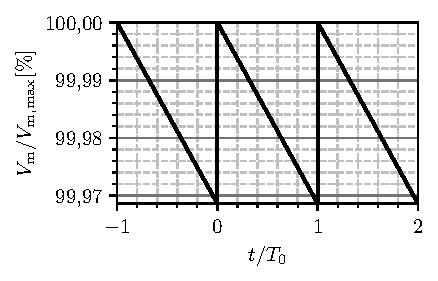
\includegraphics{fig/comb_RLC_ss.pdf}
    \caption{Релативна амплитуда у зависности од времена.}
    \label{fig:\ID.final}
\end{figure}
%
На слици \ref{fig:\ID.final} приказан је временски дијаграм релативне амплитуде 
$V_{\rm m}/V_{\rm m, max}$ на неколико периода. Амплитуда се веома споро мења јер је $\upsigma \ll \upomega$, 
па тако може да се усвоји да је амплитудска вредност практично константна и износи 
\begin{eqnarray}
    V_{\rm m} \approx \dfrac{10}{\uppi} \unit{\dfrac{V}{nC}} Q.
\end{eqnarray}
